%\documentclass[twocolumn]{article}
\documentclass[twocolumn,apj]{aastex63}
\pdfoutput=1
\usepackage{amsmath,amssymb,gensymb,color,graphicx,array,multirow,soul,rotating}
\usepackage{natbib,multirow,placeins,textcomp,subfigure}
\usepackage[outline]{contour}
%\usepackage[margin=14mm,top=10mm]{geometry}
\usepackage[utf8]{inputenc}
\usepackage[T1]{fontenc}
%\usepackage{threeparttable}
\usepackage{booktabs}
\usepackage{microtype}
%\usepackage{bm}
\usepackage{listings}
\usepackage{hyperref}

\newcommand{\planck}{{\it Planck}}
\newcommand{\wmap}{{\sl WMAP}}
\newcommand{\cobe}{{\sl COBE}}
\newcommand{\code}[1]{\texttt{#1}}

\DeclareFixedFont{\ttb}{T1}{txtt}{bx}{n}{9} % for bold
\DeclareFixedFont{\ttm}{T1}{txtt}{m}{n}{9}  % for normal
\DeclareRobustCommand{\hlblack}[1]{{\sethlcolor{black}\hl{#1}}}
\newcommand{\dfn}[1]{\textbf{#1}}
\newcommand{\img}[2][]{\resizebox{\hsize}{!}{\includegraphics[#1]{#2}}}
\newenvironment{closetabcols}[1][0.5mm]{\setlength{\tabcolsep}{#1}}{}
\newenvironment{closetabrows}[1][0.02]{\renewcommand{\arraystretch}{#1}}{}
\newcommand{\degrange}[3]{$#1^\circ < \textrm{#2} < #3^\circ$}
%\newcommand{\Earth}[0]{\oplus}
\newcommand{\cskip}{\multicolumn{1}{c}{}}
\newcommand{\ukrts}{$\micro$K$\sqrt{\text{s}}$}
\newcommand{\ukam}{$\micro$K arcmin}
%\renewcommand\Authfont{\normalsize}
%\renewcommand\Affilfont{\footnotesize}
\newcommand\skn[1]{\textcolor{blue}{SKN: #1}}

\lstset{
	language=Python,
	tabsize=2,
	basicstyle={\footnotesize\ttfamily},
	keywordstyle=\color{blue},
	commentstyle=\color{dkgreen},
	stringstyle=\color{mauve},
	breaklines=true,
	breakatwhitespace=false,
}

\begin{document}

%\title{Large-scale power loss from subtle mapmaking model errors}
%\title{Ground based CMB maps vulnerable to large-scale power loss}
%\title{Sub-pixel errors can bias the largest scales during mapmaking}
%\title{impact of sub-pixel errors on the recovery of large angular scales in CMB mapmaking}
\title{Large-scale power loss in ground-based CMB maps}

\author[0000-0002-4478-7111]{Sigurd~Naess}
\affil{Institute of Theoretical Astrophysics, University of Oslo, Norway}

\keywords{}

\begin{abstract}
\vspace*{5mm}
\end{abstract}

\section{Introduction}
\skn{Should cite \citet{model-error}. Should say something about discussion about
this in the literature being limited to high-contrast regions, and cite XGLS
etc.}

CMB telescopes observe the sky by scanning their detectors across
it while continuously reading off a series of samples from the
detectors. Typically the signal-to-noise ratio of each sample is
small, but by combining a large number of samples with knowledge
of which direction the telescope was pointing at any time, it's
possible to reconstruct an image of the sky. There are several
ways of doing this, with the most common being maximum-likelihood,
filter+bin and destriping. These all start by modelling the
telescope data as
\begin{align}
	d = Pm + n \label{eq:model}
\end{align}
where $d$ is the set of samples read off from the detectors
(often called the time-ordered data), $m$ is the set of pixels
of the sky image we want to reconstruct, $n$ is the noise
in each sample (usually with significant correlations), and
$P$ is a pointing matrix that encodes how each sample responds
to the pixels in the image.

Given the model, it's possible to either directly solve for
an unbiased map (as in maximum likelihood mapmaking or destriping),
or to measure and correct for the bias in a biased estimator
(as in filter+bin mapmaking). However, this fails when the model
does not actually describe the data, and this turns out to be
the norm rather than the exception. The goal of this paper is to
demonstrate the unintuitive and surprisingly large (O(1)) effect
even seemingly inconsequential model errors can have when imaging
the CMB. The full scope of these erorrs appears to be largely
unappreciated, and I fear that most ground-based CMB analyses
so far suffer from uncorrected bias at low multipoles in total intensity
due to these effects.

\section{Subpixel errors}
Subpixel errors may be both the most common and most important
class of model errors in CMB mapmaking.
For efficiency reasons $P$ is always\footnote{I am not aware of any
published CMB analysis that has done something else.}
chosen to use simple nearest-neighbor interpolation, where the
value of a sample is simply given by the value of the pixel nearest
to it. This means that $P$ can be implemented by simply reading off
one pixel value per sample, and its transpose $P^T$ consists of simply
summing the value of the samples that hit each pixel. However, this
comes at the cost of there being a discontinuous jump in values as one
scans from one pixel to the next, as illustrated in figure~\ref{fig:nearest-neigh}.
Hence, the closest the model can get to a smooth curve is a
staircase-like funciton that hugs it, leaving a residual full of
discontinuous jumps (the blue curve in the figure).

Discontinuous residuals are not necessarily problematic. The trouble arises
when this is coupled with a likelihood\footnote{The equivalent for filter+bin is a filter that
impacts some modes more than others (which is the whole point of a filter),
and for destriping it's a baseline amplitude prior with those properties.
} where some modes have much less weight than others. Ground-based CMB
telescopes suffer from atmospheric emission that acts as a large source
of noise on large scales. This leads to time-ordered data noise power
spectra similar to the one sketched in figure~\ref{fig:ps}, with
a white noise floor at short timescales (high frequency) transitioning to a steep
rise of several orders of magnitude as one moves to longer timescales
(low frequency). In this case long-wavelength modes have orders of magnitude
lower weight in the likelihood than short-wavelength modes. Put another way,
they are orders of magnitude \emph{cheaper to sacrifice} when the model can't fully
fit the data.

\begin{figure*}
	\centering
	\begin{tabular}{cc}
		\dfn{\large a} & \dfn{\large b} \\
		\raisebox{-0.5\height}{\includegraphics[height=70mm]{nearest_neigh/path.pdf}} &
		\hspace*{-5mm}\raisebox{-0.5\height}{\includegraphics[height=70mm]{nearest_neigh/vals.pdf}}
	\end{tabular}
	\caption{
		\dfn{a}: Example path (red) of a detector across a few pixels.
		The area closest to each pixel center (black dots) is shown with dotted lines.
		In the nearest neighbor model, the value associated with each sample is simply
		that of the closest pixel, regardless of where inside that pixel it is.
		\dfn{b}: Example detector signal (red) for the same path. The closest
		matching model (green) leaves a jagged residual (blue) that has power on
		all lengthscales despite the signal itself being very smooth.
		For comparison, if our model were a constant zero, then the residual
		would just be the signal itself (red), and hence smooth.
		{\bf If smooth residuals are much cheaper in the likelihood than jagged ones,
		then a zero model will be preferred to one that hugs the signal as
		tightly as possible} like the green curve.
	}
	\label{fig:nearest-neigh}
\end{figure*}

\begin{figure}
	\centering
	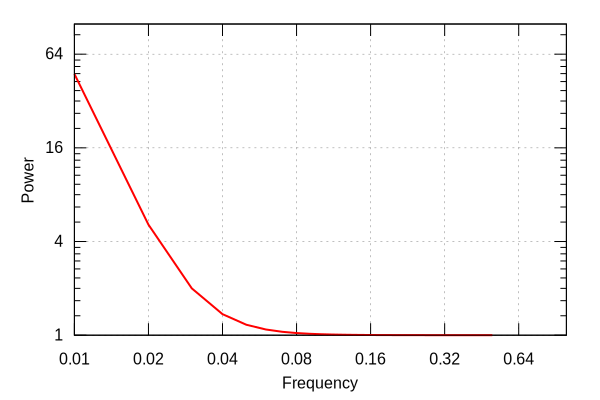
\includegraphics[width=\columnwidth]{subpix/ps.pdf}
	\caption{
		The noise model/inverse weights/inverse filter used in the subpixel
		bias demonstration in figures~\ref{fig:subpix-bias} and \ref{fig:subpix-noerr}.
		It is a simple Fourier-diagonal 1/f + white noise spectrum
		typical for ground-based CMB observations. The frequency axis is in
		dimensionless units in this toy example, but for real telescopes the
		transition from white noise is typically a few Hz, corresponding
		to multipoles of hundreds on the sky.
	}
	\label{fig:ps}
\end{figure}

\subsection{Toy example}
To illustrate the interaction between a nearest neighbor pointing matrix's
subpixel errors and a likelihood where large scales have low weight, let
us consider a simple 1D case where 100 samples scan uniformly across 10 pixels:
\begin{lstlisting}
npix  = 10
nsamp = 100
pix   = np.arange(nsamp).astype(float)*npix/nsamp
\end{lstlisting}
A standard nearest-neighbor pointing matrix for this looks like:
\begin{lstlisting}
P = np.zeros((nsamp,npix))
for i, p in enumerate(pix):
	P[i,int(np.round(pix[i]))%npix] = 1
\end{lstlisting}
We build the inverse noise matrix/filter/baseline-prior $F$ by
projecting an inverse fourier spectrum into pixel space:
\begin{lstlisting}
freq   = np.fft.rfftfreq(nsamp)
inv_ps = 1/(1+(np.maximum(freq,freq[1]/2)/0.03)**-3.5)
F = np.zeros((nsamp,nsamp))
I = np.eye(nsamp)
for i in range(nsamp):
	F[:,i] = np.fft.irfft(inv_ps*np.fft.rfft(I[i]), n=nsamp)
\end{lstlisting}
The signal itself consists of just a long-wavelength sine wave:
\begin{lstlisting}
signal = np.sin(2*np.pi*pix/npix)
\end{lstlisting}
With this in place, we can now define our map estimators.

\subsubsection{Binning}
The \emph{binned map} is simply the mean value of the samples
in each pixel, with no weighting:
\begin{lstlisting}
map_binned = np.linalg.solve((P.T.dot(P)), P.T.dot(signal))
\end{lstlisting}
:%s
\subsubsection{Maximum-likelihood}
The maximum-likelihood solution of equation~\ref{eq:model} for the
sky image $m$ is
\begin{align}
	\hat m = (P^TN^{-1}P)^{-1}P^TN^{-1}d
\end{align}
where $N$ is the covariance matrix of the noise $n$.
In our toy example, $N^{-1} = F$, so the \emph{maximum-likelihood map}
is
\begin{lstlisting}
map_ml = np.linalg.solve((P.T.dot(F).dot(P)),P.T.dot(F.dot(signal)))
\end{lstlisting}

\subsubsection{Filter+bin}
As the same suggests, filter+bin consists of filtering the time-ordered
data, and then making a binned map. We'll use $F$ as our filter, so
the \emph{filter+bin map} is
\begin{lstlisting}
map_fb = np.linalg.solve(P.T.dot(P), P.T.dot(F).dot(signal))
\end{lstlisting}
The filter+bin map is biased by design, so to interpret or debias it one
needs to characterize this bias. There are two common approaches
to doing this: Observation matrix and simulations.

\paragraph{Observation matrix}
The observation matrix approach (cite BICEP here)
recognizes that the whole chain of operations observe, filter, map
together make up a linear system, and can therefore be represented
as a matrix, called the \emph{observation matrix}. Building this matrix is heavy, but doable for some
surveys. Under the standard assumption that the observation step is
given by equation~\ref{eq:model}, the observation matrix is given by
\begin{lstlisting}
obsmat = np.linalg.inv(P.T.dot(P)).dot(P.T.dot(F).dot(P))
\end{lstlisting}
and using it, we can define a debiased filter+bin map
\begin{lstlisting}
map_fb_deobs = np.linalg.solve(obsmat, map_fb)
\end{lstlisting}

\paragraph{Simulations}
Alternatively, and more commonly, one can characterize the bias
by simulating the observation of a set of random skies, passing
them through the filter+bin process, and comparing the properties
of the input and output images. The standard way of doing this is
by assuming that equation~\ref{eq:model} describes the observation
process, and that the bias can be described by a \emph{transfer function}:
a simple independend scaling of each fourier mode. Under
these assumptions, we can measure and correct the bias as follows.
\begin{lstlisting}
nsim = 1000
sim_ips = np.zeros(npix//2+1)
sim_ops = np.zeros(npix//2+1)
for i in range(nsim):
	sim_imap = np.random.standard_normal(npix)
	sim_omap = np.linalg.solve(P.T.dot(P), P.T.dot(F).dot(P).dot(sim_imap))
	sim_ips += np.abs(np.fft.rfft(sim_imap))**2
	sim_ops += np.abs(np.fft.rfft(sim_omap))**2
tf = (sim_ops/sim_ips)**0.5
map_fb_detrans = np.fft.irfft(np.fft.rfft(map_fb)/tf, n=npix)
\end{lstlisting}

\subsubsection{Destriping}
Destriping splits the noise into a correlated and uncorrelated part,
and models the correlated noise as as a series of slowly changing
degrees of freedom to be solved for jointly with the sky image itself.
The data is modeled as
\begin{align}
	d &= Pm + Qa + n_w
\end{align}
where $n_w$ is the white noise with diagonal covariance matrix $N_w$,
and $Q$ describes how each correlaetd noise degree of freedom $a$
maps onto the time-ordered data, typically in the form of seconds
(ground) to minutes (space) long baselines. Given this, the
maximum-likelihood solutions for $a$ and $m$ are
\begin{align}
	Z &= I - P(P^TN_w^{-1}P)^{-1}P^TN_w^{-1} \notag \\
	a &= (Q^TN_w^{-1}ZQ + C_a^{-1})^{-1} Q^TN_w^{-1}Zd \notag \\
	m &= (P^TN_w^{-1}P)^{-1}P^TN_w^{-1}(d - Qa)
\end{align}
where $C_a$ is one's prior knowledge of the covariance of $a$.
Destriping allows a speed/optimality tradeoff in the choice of
baseline length and prior, and approaches the maximum likelihood
map when the baseline length is a single sample and $C_a + N_w = N$.
We implement this limit below. In our toy example $N_w = I$, so $C_a = F^{-1}-I$.
\begin{lstlisting}
iCa = np.linalg.inv(np.linalg.inv(F) - I)
Z   = I-P.dot(np.linalg.solve(P.T.dot(P), P.T))
a   = np.linalg.solve(Z+iCa, Z.dot(signal))
map_ds = np.linalg.solve(P.T.dot(P), P.T.dot(signal - a))
\end{lstlisting}
\skn{refs and citations from https://arxiv.org/pdf/1103.2281.pdf}

\subsubsection{Results}
\begin{figure}
	\centering
	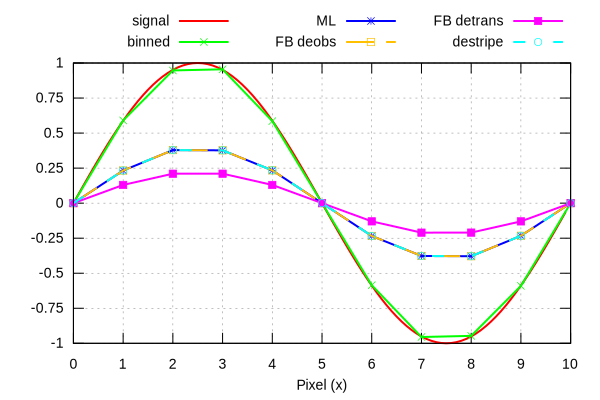
\includegraphics[width=\columnwidth]{subpix/model_error_toy.pdf}
	\caption{
		Demonstration of large loss of power in long-wavelength mode
		caused by the poor subpixel treatment in the standard nearest-neighbor pointing matrix.
		Figure~\ref{fig:ps} shows the noise model/inverse weights/inverse filter
		used in the various methods.
		\dfn{signal}: The input signal, a smooth long-wavelength mode,
		sampled at 10 samples per output pixel.
		\dfn{binned}: Simple binned map (the unweighted average per pixel).
		Very suboptimal in the presence of correlated noise, but unbiased.
		\dfn{ML}: Maximum-likelihood map. 2/3 of the signal is lost despite
		the naive expectation of biaslessness for this estimator.
		\dfn{FB deobs}: Filter+bin map debiased using an observation matrix.
		Identical to ML.
		\dfn{FB detrans}: Filter+bin map debiased by deconvolving a
		transfer function measured from simulations. Even more biased
		than the others due to ignoring mode coupling.
		\dfn{destripe}: Destriper in the limit of 1-sample baselines.
		Identical to ML.
	}
	\label{fig:subpix-bias}
\end{figure}

Figure~\ref{fig:subpix-bias} compares the recovered 1D sky ``images''
for the different mapmaking methods for this toy example.

\begin{figure}
	\centering
	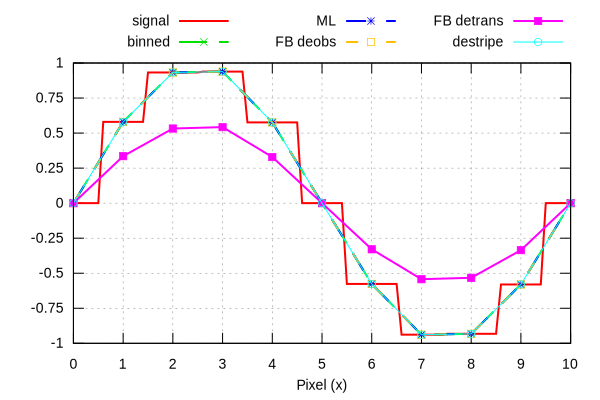
\includegraphics[width=\columnwidth]{subpix/model_error_toy_noerr.pdf}
	\caption{
		Like figure~\ref{fig:subpix-bias}, but with the input signal
		having the same nearest-neighbor pixelization as the models.
		In this case all models except FB detrans are unbiased.
	}
	\label{fig:subpix-noerr}
\end{figure}

\begin{figure}
	\centering
	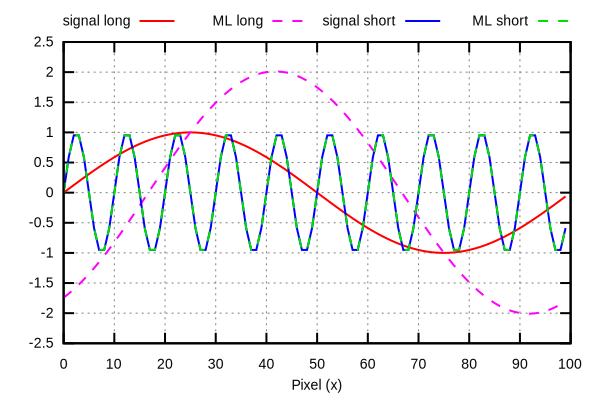
\includegraphics[width=\columnwidth]{common_mode/common.pdf}
	\caption{
		Demonstration of large-scale bias in a multi-detector system
		due to an interaction between strong large-scale
		detector correlations in the noise model and large
		relative gain errors between the detectors.
		\dfn{signal long}: An input long-wavelength signal,
		with the same pixelization as the output to avoid subpixel bias.
		\dfn{ML long}: Corresponding maximum-likelihood map, which
		exhibits both an amplitude and phase error.
		\dfn{signal short} and \dfn{ML short}: The same, but for a
		short-wavelength mode. Here the bias is negligible,
		despite the model's gain errors being scale-independent.
	}
	\label{fig:common}
\end{figure}

\bibliographystyle{act_titles}
\bibliography{refs}

\end{document}
